\titre{Définition :} Logiciel ou boitier matériel conçu pour filtrer les échanges de données entre un réseau / une application de confiance et une réseau / une application extérieur. \\

\titre{Couches concernées :} 
	\begin{itemize}
		\item entête Réseau (IP)
		\item entête Transport (TCP, UDP)
		\item charge utile (filtrage d'url, type de fichier)
	\end{itemize}
On peut placer un pare feu en entrée d'un réseau de confiance et/ou en entrée d'une machine.\\

\titre{Rappel : Connexion http classique} \\
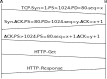
\includegraphics[width=300px]{Images/17_Http.pdf} \\
Autorisation de filtrage dans B:
\begin{enumerate}
	\item Autoriser PS>1024, PD=80, SYN=1
	\item Autoriser PS=80, PD>1024, SYN=1, ACK=1, @IP-B, @IP-A(toutes du réseau autorisé) 
	\item Autoriser PS>1024, PD=80, ACK=1, @IP-A(toutes du réseau autorisé) @IP-B
	\item Autoriser PS=80, PD>1024, ACK=1, @IP-B, @IP-A(toutes du réseau autorisé) 
\end{enumerate}

\titre{Historique :} 
	\begin{itemize}
		\item Filtrage statique : ils n'avaient pas de mémoire pour enregistrer l'état d'une connexion (on ne peut pas vérifier les numéros de séquence par exemple). Ce type de filtre est plus efficace en bloquage qu'en autorisation.
		\item Proxy : Apparu en même temps que le filtrage statique. A l'époque, ils ont été créés pour économiser les adresses IP (avant, les IP étaient organisées par classes). Le proxy permet de donner un accès au web à toutes les machines d'un réseau local avec une seule adresse publique. Puisque toutes les requêtes passent par lui, il peut les filtrer. Actuellement les proxy sont encore utilisés comme serveurs de cache, filtres d'url et de contenu.\\
			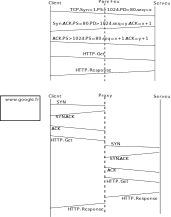
\includegraphics[width=300px]{Images/18_Proxy.pdf} \\
			Il faut un Proxy par type d'application car il doit connaitre les protocoles de la couche application (ex: HTTP). \\
			Cas particulier : les proxy socks : \\ \begin{tabular}{|c|c|c|c|} \hline IP & UDP & \begin{tabular}{l} Socks \\ @client \\ @serveurfinal \\ @serveursocks \\ protocole transport \\ port dest \end{tabular} & HTTP-GET \\ \hline\end{tabular}
		\item Filtrage dynamique (autorise le premier paquet, et ceux qui suivent logiquement). Le pare feu possède une mémoire qui enregistre un suivi de connexion. \\ 
		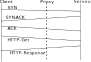
\includegraphics[width=170px]{Images/19_FiltrageDynamique.pdf}
		\begin{tabular}{|l|} \hline
			Table de suivi de connexion \\ \hline
			IP-S = IP-A \\ \hline
			IP-Dest = IP-B \\ \hline
			Port-Source = 1025 \\ \hline
			Port-Dest = 80 = \\ \hline
			Num Seq = \\ \hline
			Num ACK = \\ \hline
			SYN = 1 \\ \hline
		\end{tabular} \\ \\
		Lorsque le pare feu reçoit la réponse il l'examine et vérifie que tous les champs sont en correspondance dans la mémoire. \\
		Remarque : puisque le pare feu doit enregistrer les IP et les ports, c'est généralement sur lui qu'on implémente la translation d'adresses. 

	\end{itemize}

\titre{Rappel : Translation d'adresse} Elle sert à palier la pénurie d'adresses IP publiques.\\
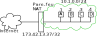
\includegraphics[width=250px]{Images/20_NAT.pdf}\\
Scénario : 
\begin{itemize}
	\item A envoie : \\|4 \ldots|10.1.0.1|1.2.3.4|1025|80|\ldots| à l'adresse IP 1.2.3.4.
	\item Le paquet est transformé : \\|4 \ldots|173.42.13.37|1.2.3.4|1025|80|\ldots|
	\item B envoie : \\|4 \ldots|10.1.0.2|1.2.3.4|1025|80|\ldots| à l'adresse IP 1.2.3.4.
	\item Le paquet est transformé : \\|4 \ldots|173.42.13.37|1.2.3.4|1026|80|\ldots| à l'adresse IP 1.2.3.4.
	\item 1.2.3.4 répond : \\|4 \ldots|1.2.3.4|173.42.13.37|80|1025|\ldots|
	\item Le pare feu sait que c'est pour A grâce au port-dest 1025.
	\item Le paquet est transformé et renvoyé à A : \\|4 \ldots|1.2.3.4|10.1.0.1|80|1025|\ldots|
	\item 1.2.3.4 répond : \\|4 \ldots|1.2.3.4|173.42.13.37|80|1026|\ldots|
	\item Le pare feu sait que c'est pour B grâce au port-dest 1026.
	\item Le paquet est transformé et renvoyé à A : \\|4 \ldots|1.2.3.4|10.1.0.2|80|1025|\ldots|
\end{itemize}

\begin{tabular}{|l|l|l|l|} \hline
	\multicolumn{2}{|l|}{Interne} & Externe \\ \hline
	IP-Src & Port-Src & Port-Src\\ \hline
	10.1.0.1 & 1025 & 1025 \\ \hline
	10.1.0.2 & 1025 & 1026 \\ \hline
\end{tabular}

En lui même, le translateur d'adresses constitue déjà une sécurité, car une machine à l'extérieur du réseau privé ne peut pas contacter une machine à l'intérieur si la machine à l'intérieur n'a pas initié de connection. \\
Si on veut héberger un serveur dans le réseau interne, il faut saisir manuellement une ligne IP-Serveur, Port 80, Port 80 dans la table de translation et autoriser les connections entrantes sur le port 80. \\
Problème : Un pirate qui accède à notre serveur http entre dans le réseau local, de là il peut potentiellement accéder aux autres machines du même réseau. Il faut un autre pare feu entre les serveurs et le reste du réseau local. \\

\includegraphics[width=150px]{Images/21_DMZ.pdf}
\includegraphics[width=100px]{Images/22_DMZ.pdf}\\

\titre{Reverse Proxy :} Serveurs cache spécialisés dans l'hébergement web. Ils vont avoir 2 rôles : 
	\begin{itemize}
		\item Augmenter la sécurité et la fiabilité
		\item Faire de la répartition de charge
	\end{itemize}

\includegraphics[width=150px]{Images/23_ReverseProxy.pdf}\\

\titre{SYN Flooding : } Déni de service (peut être coupé par un pare-feu dynamique mais pas simple)
